In this section, we describe the data that we analyse and how we aggregate goods and services to 8 consumption composites.

\subsection{Household budget survey data}
We obtain data on household consumption from the Danish Household Budget Survey, which have been compiled annually since 1994 \citep{hhbudgetsurvey}. The data describes annual consumption in private households, divided into consumption of almost 1300 goods and services. The survey is based on a combination of interviews, accounting and administrative data from participating households, and the population covers all private households in Denmark. \cite{hhbudgetsurvey} defines a private household as \textit{"an economic unit, i.e. a group of people who live together an have a high degree of common economy, i.e. share income and expenses."}. The survey covers between 2000 and 3000 households each year.

Our dataset is aggregated to deciles of disposable income of the main income recipient of a given household. 

\begin{table}[]
\caption{Descriptive statistics, household budget surve data (2019)}
\label{descstat}
\resizebox{\textwidth}{!}{
\begin{tabular}{llllllllllll}
                                    &       & \multicolumn{10}{c}{Decile}                                 \\ \cline{3-12} 
                                    & Total & 1   & 2   & 3   & 4   & 5   & 6   & 7   & 8   & 9   & 10    \\ \hline
Households in the survey            & 2.166 & 180 & 208 & 205 & 222 & 177 & 174 & 228 & 247 & 247 & 278   \\
Households in DK                    & 2.761 & 316 & 321 & 311 & 287 & 229 & 235 & 251 & 268 & 264 & 279   \\
Average \# of persons in household  & 2.1   & 1.8 & 1.8 & 1.9 & 2.0 & 2.5 & 2.5 & 2.3 & 2.2 & 2.2 & 2.1   \\ \hline
Avg. Disposable income (1000 DKK)   & 459   & 159 & 233 & 278 & 334 & 440 & 488 & 511 & 573 & 683 & 1,015 \\
Avg. Total expenditure (1000   DKK) & 323   & 198 & 220 & 234 & 275 & 318 & 353 & 358 & 382 & 433 & 520  \\ \hline
\end{tabular}}
    \captionsetup{singlelinecheck=off,size=scriptsize}
\setlength{\captionmargin}{10pt}
\caption*{
\textbf{Source:} Household budget survey, \cite{hhbudgetsurvey}.}
\end{table}

Our raw data set describes consumption of almost 1300 goods and services for each decile and each year from 1994-2019. We aggregate these to 282 groups for which we have price indices in the sample period. For example, this means that rice, rice pudding etc. and rice dishes is aggregated into one category called 'rice' by the sum of the consumption of each of the goods. 

There is a small tendency towards underrepresentation of the lower income deciles in the survey, as per table \ref{descstat}. To ensure both better representativeness and less volatile consumption series, we aggregate these deciles to quintiles, such that decile 1 and 2 is aggregated to quintile 1 and so forth.

\subsection{Income, expenditure and savings}
The five quintiles have very different savings behavior. As can be seen from figure \ref{fig:inccons} and \ref{fig:savings}, disposable income has been increasing for all quintiles, and in general, savings have been increasing as well. However, the bottom quintile has on average negative savings for almost all of the sample period, while the richest quintile has increased their savings rate from an already high level. It should be noted that the bottom quintile of the income distribution includes households with large negative income due to losses on stocks and business ownership, which drives the average income down \cite[IFOR32]{statbank}. This may help explain the somewhat large negative savings rate for the bottom quintile, which at one point in 2007 was at -67 pct. 

All quintiles have increased their savings rate in the sample period, and the richer quintiles have higher savings rates than the bottom quintiles. This is consistent with the stylized fact that the richer people get, the more they tend to save out of their income \citep{dynan2004rich}.
\begin{figure}[H]
\centering
\caption{Real disposable income and total real expenditure}
\label{fig:inccons}
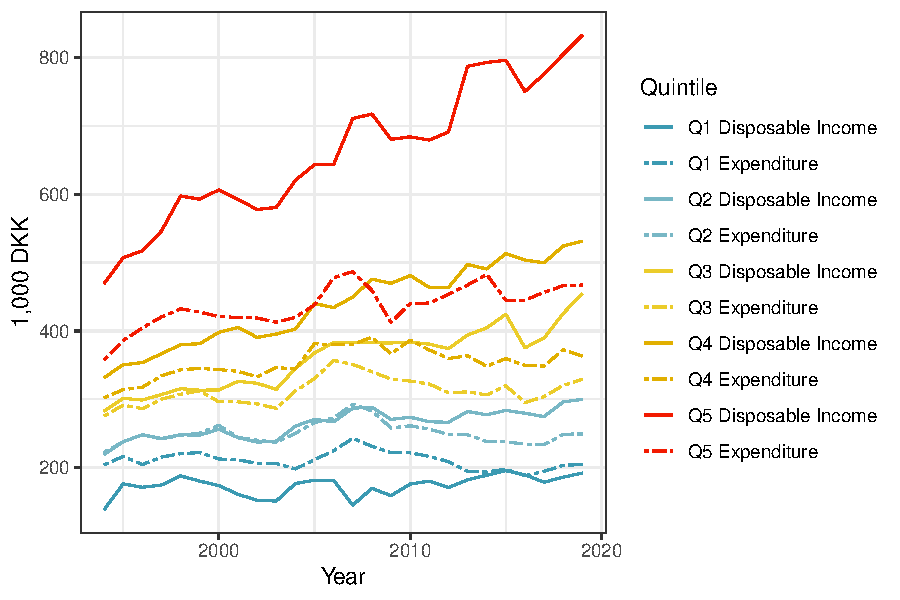
\includegraphics[width=.8\textwidth]{Figures/forb_indk.pdf}
\captionsetup{singlelinecheck=off,size=scriptsize}
\setlength{\captionmargin}{10pt}
\caption*{
\textbf{Note:} Disposable income and total expenditure is deflated with the consumer price index. \citep[PRIS112]{statbank}}
\end{figure}

\begin{figure}[H]
\centering
\caption{Savings rates}
\label{fig:savings}
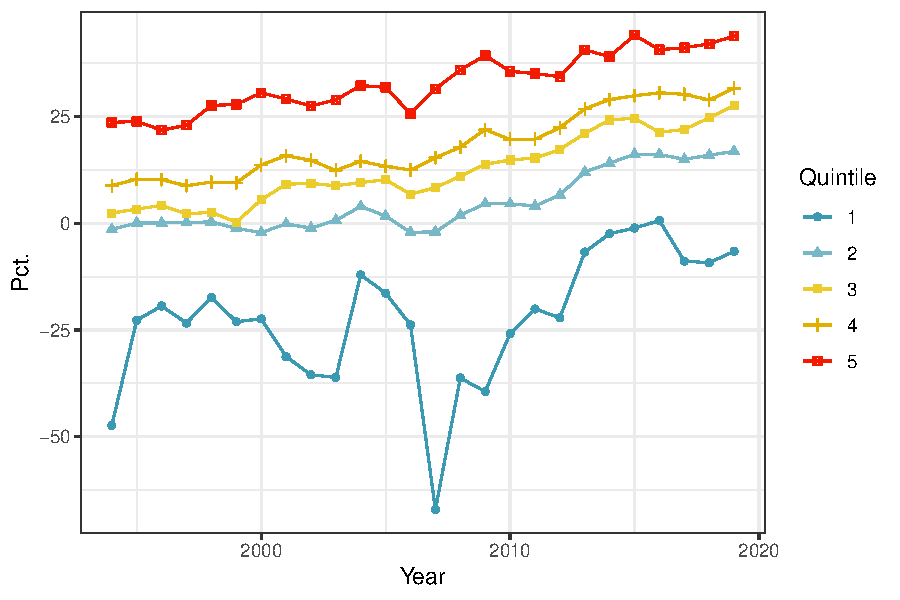
\includegraphics[width=.8\textwidth]{Figures/savings.pdf}
\captionsetup{singlelinecheck=off,size=scriptsize}
\setlength{\captionmargin}{10pt}
\caption*{
\textbf{Note:} ??\\}
\end{figure}

\subsection{Aggregation to 8 consumption composites}\label{sec:consgroups}
In our estimation of the linear expenditure system, the numbers of estimated parameters increase exponentially in the number of consumption categories, as we estimate a covariance matrix for the error terms, see section \ref{sec:estimationequation}. To keep the estimation 
manageable for the numeric solver in R, we can only estimate the system for a limited number of goods. Through experiments, we find that 8 consumption composites is a desirable trade-off between a reasonably low number of goods and separation of the most relevant consumption groups, such that we single out the most carbon-intensive We aggregate from the 282-level to 8 consumption composites. The groups are partly based on the consumption aggregates that Statistics Denmark provide themselves as well as the consumption aggregates in \cite{makroforbrug2020}, but with notable exceptions, mostly that meat and dairy, energy for housing and energy for transport are singled out. 
\begin{enumerate}
  \item \textbf{Meat and dairy:} Beef, pork, chicken, other meats, seafood, dairy products and eggs.
  \item \textbf{Other foods:} Rice, flour, bread, pasta, other grains and grain products, vegetable oils, fruit and vegetables, sugar, sweets, coffee, tea, ready meals, soft drinks, cigarettes and alcohol.
  \item \textbf{Housing:} Rent, imputed rent, maintenance and repair of dwelling, other dwelling-related services, water supply
  \item \textbf{Energy for housing:} Electricity, natural gas, petroleum for heating, coal, district heating
  \item \textbf{Energy for transport:} Gasoline, diesel, other fuels, lubricants for cars
  \item \textbf{Transport}: New and used cars, motorcycles, bicycles, passenger transport with train, bus, taxi, ferry, domestic and international flights, other transport services
  \item \textbf{Other goods:} Clothes, shoes, furniture and other furnishings,  household appliances, tools, medicine, glasses, hearing aid, electric appliances, software, games and toys, newspapers, books, etc.
  \item \textbf{Other services:} Clothing services, medical services, household services, dental, communication services, recreational services, restaurants, package holidays, restaurants and hotels, hairdressing, insurance and other financial services.
\end{enumerate}
The production of meat (especially beef and lamb) and dairy is generally associated with a higher carbon footprint than other foods \citep{denstoreklimadatabase}, which is why we separate food consumption into two consumption composites. The price of meat and dairy has played a prominent role in the Danish political debate on carbon taxation \citep{kodsovsellerkaos}.  Politicians worry that low-income families will not be able to afford beef if carbon pricing is too high. A recent survey showed that a significant majority of the Danish population is against increased taxes on beef and dairy as a part of a green transition \citep{megafonpolitiken}. The same survey showed that a majority is also against raising the tax on gasoline by 1 DKK/litre. Thus, we also single out gasoline and diesel consumption, also because it accounts for a large share of total expenditure by itself. Energy for housing is also a consumption category that is associated with significant carbon emissions, though emissions from electricity are expected to fall towards 2030, see section \ref{sec:kf21fremskriv}.

We plot the consumption shares of the 8 consumption groups for each quintile in figure \ref{figshare}. The lower income quintiles spend larger shares of total consumption on what we may deem 'necessities', that is meat and dairy, other foods, housing and energy for housing. It is also evident that the share of expenditure spent on food has been growing over the sample period, where income has grown quite significantly, consistent with Engel's law. At the same time, there has been an upward trend in the share of expenditure devoted to housing as well as energy for housing.

The richer income quintiles devote a larger share of expenditure to transport as well as energy for transport.  This may indicate that these consumption composites luxury goods, or it may reflect that richer quintiles own more cars, tend to live further from their workplace or otherwise have higher private transportation needs than poorer quintiles. 

The richer quintiles also generally spend a larger share of total expenditure on other goods, and to a higher degree, on other services. The share of other goods has decreased quite drastically from an average about 21 percent in the start of the sample period to only 15 pct in 2019. The spending on other services has increased, indicating that this consumption composite includes services that could be characterised as "luxurious". 
\begin{figure}[H]
\centering
\caption{Consumption shares across quintiles }
\label{figshare}
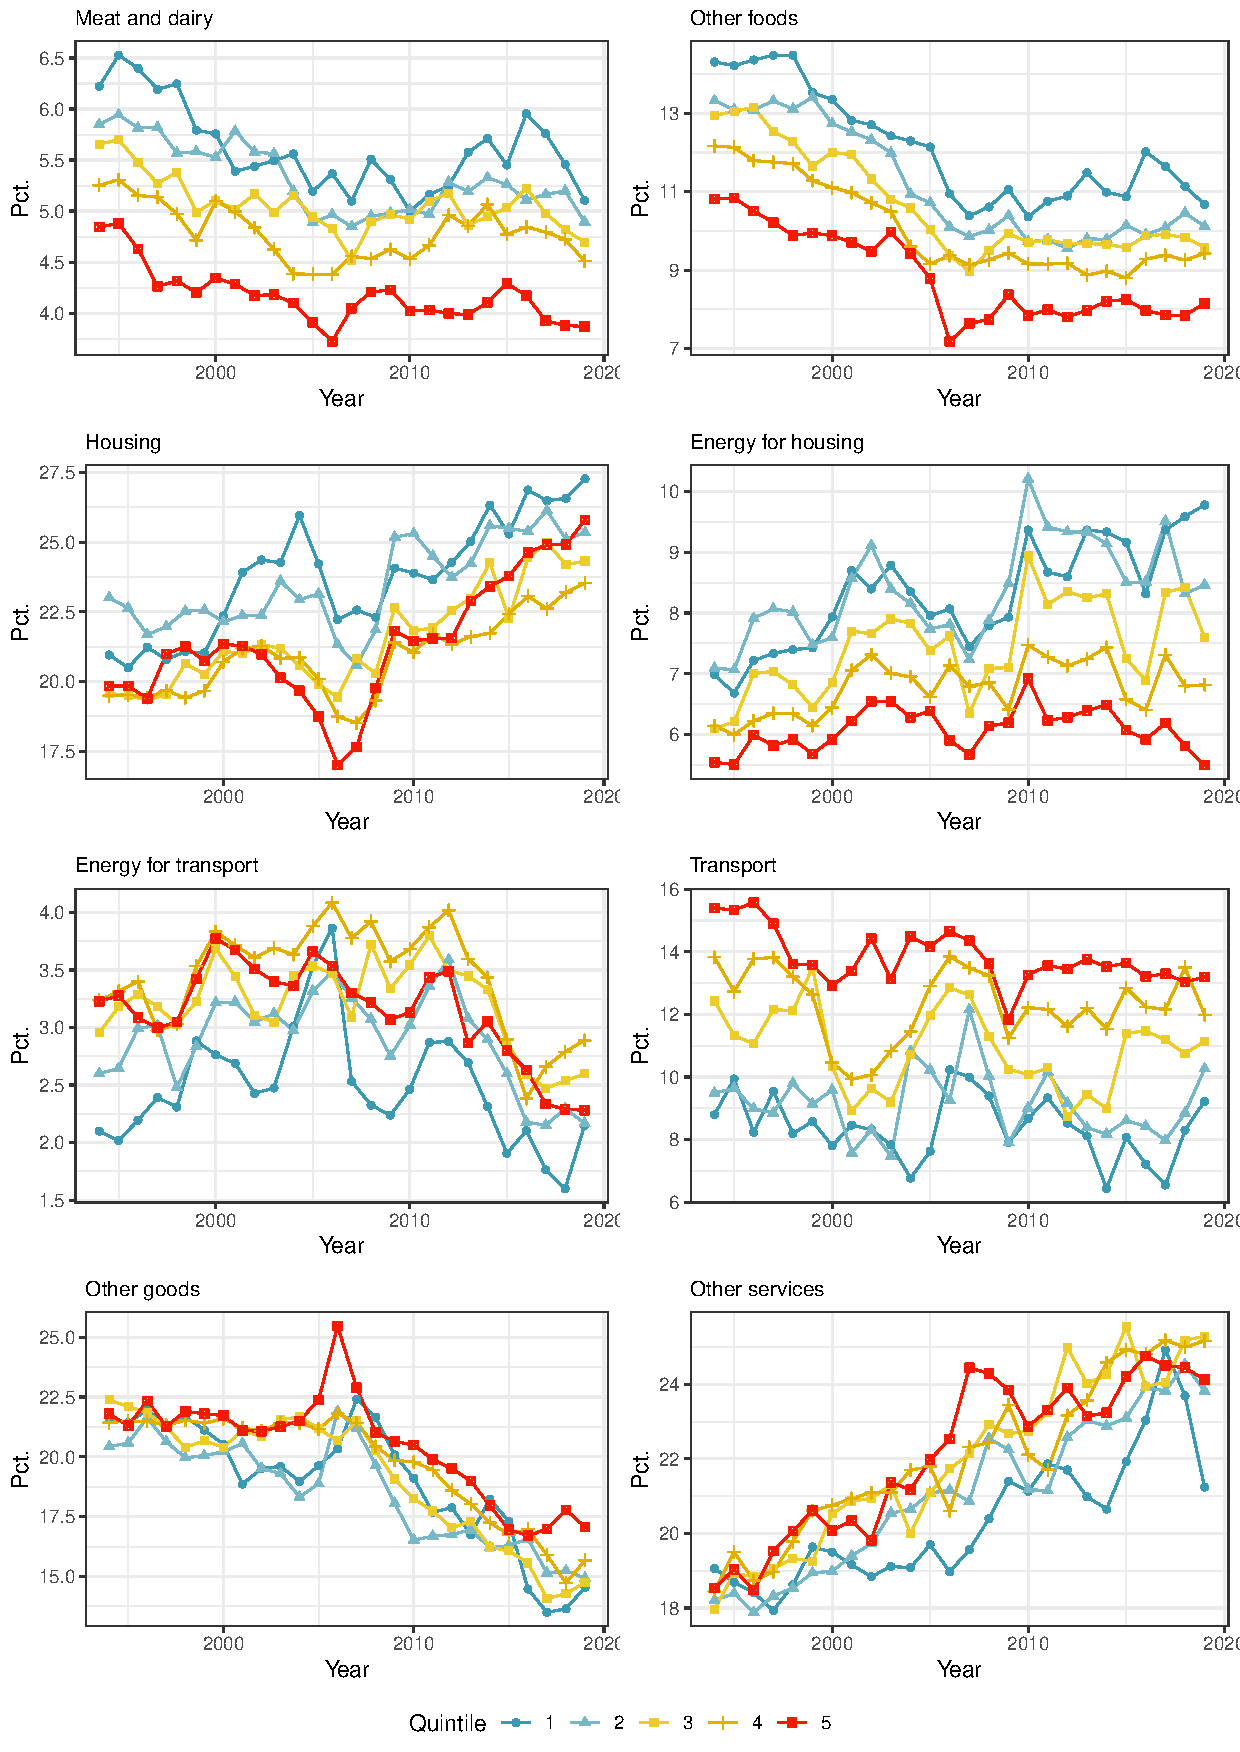
\includegraphics[width=.8\textwidth]{Figures/shareplot_quintiles.pdf}
\captionsetup{singlelinecheck=off,size=scriptsize}
\setlength{\captionmargin}{10pt}
\caption*{
\textbf{Note:} The graph depicts nominal budget shares.}
\end{figure}

Prices are calculated as a weighted average of the prices for each of the goods that make op a consumption composite. Weights are from the average household. The evolution in the prices over the sample period is shown in figure \ref{pricesfigure}. Most notably, the price of energy for transport as well as energy for housing has increased significantly over the period. The price of other services has also increased compared to other goods, consistent with the predictions of Baumol's cost disease. The price of the housing composite has also increased quite a bit over time, which can help explain how the expenditure share of that composite has also risen for all quintiles. 

\begin{figure}[H]
\centering
\caption{Price indices of the consumption composites }
\label{pricesfigure}
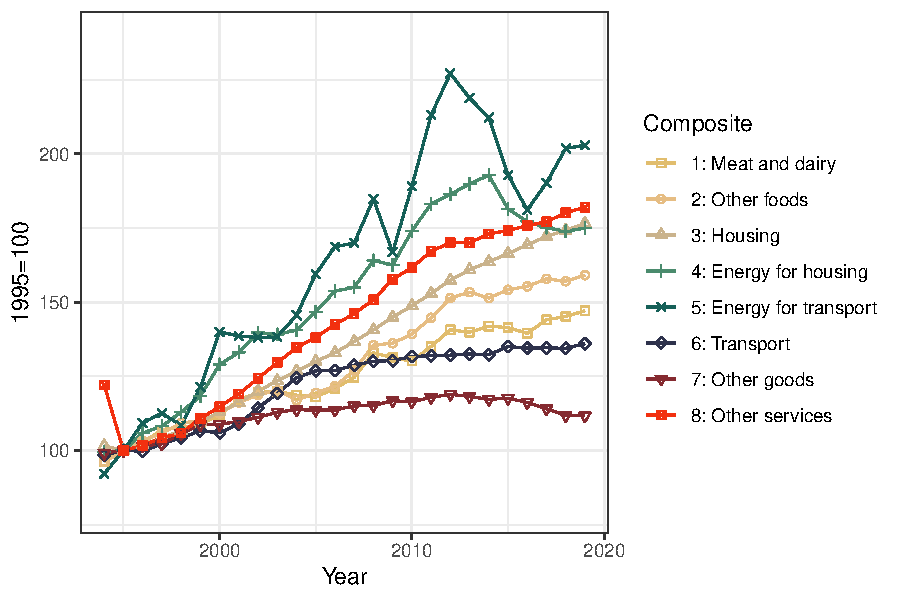
\includegraphics[width=.8\textwidth]{Figures/priceplot.pdf}
\captionsetup{singlelinecheck=off,size=scriptsize}
\setlength{\captionmargin}{10pt}
\caption*{
\textbf{Note:} Year 1995 is index 100.}
\end{figure}

To graphically assess the relationship between prices and consumption, these are plotted as indices in figure \ref{priceandrealcons}. For the food composites, we see that the price has risen as real consumption of other foods has been falling a bit for all quintiles, while real consumption of meat and dairy has been falling for lower quintiles but stayed approximately constant for upper quintiles. 


\begin{figure}[H]
\centering
\caption{Prices and real consumption}
\label{priceandrealcons}
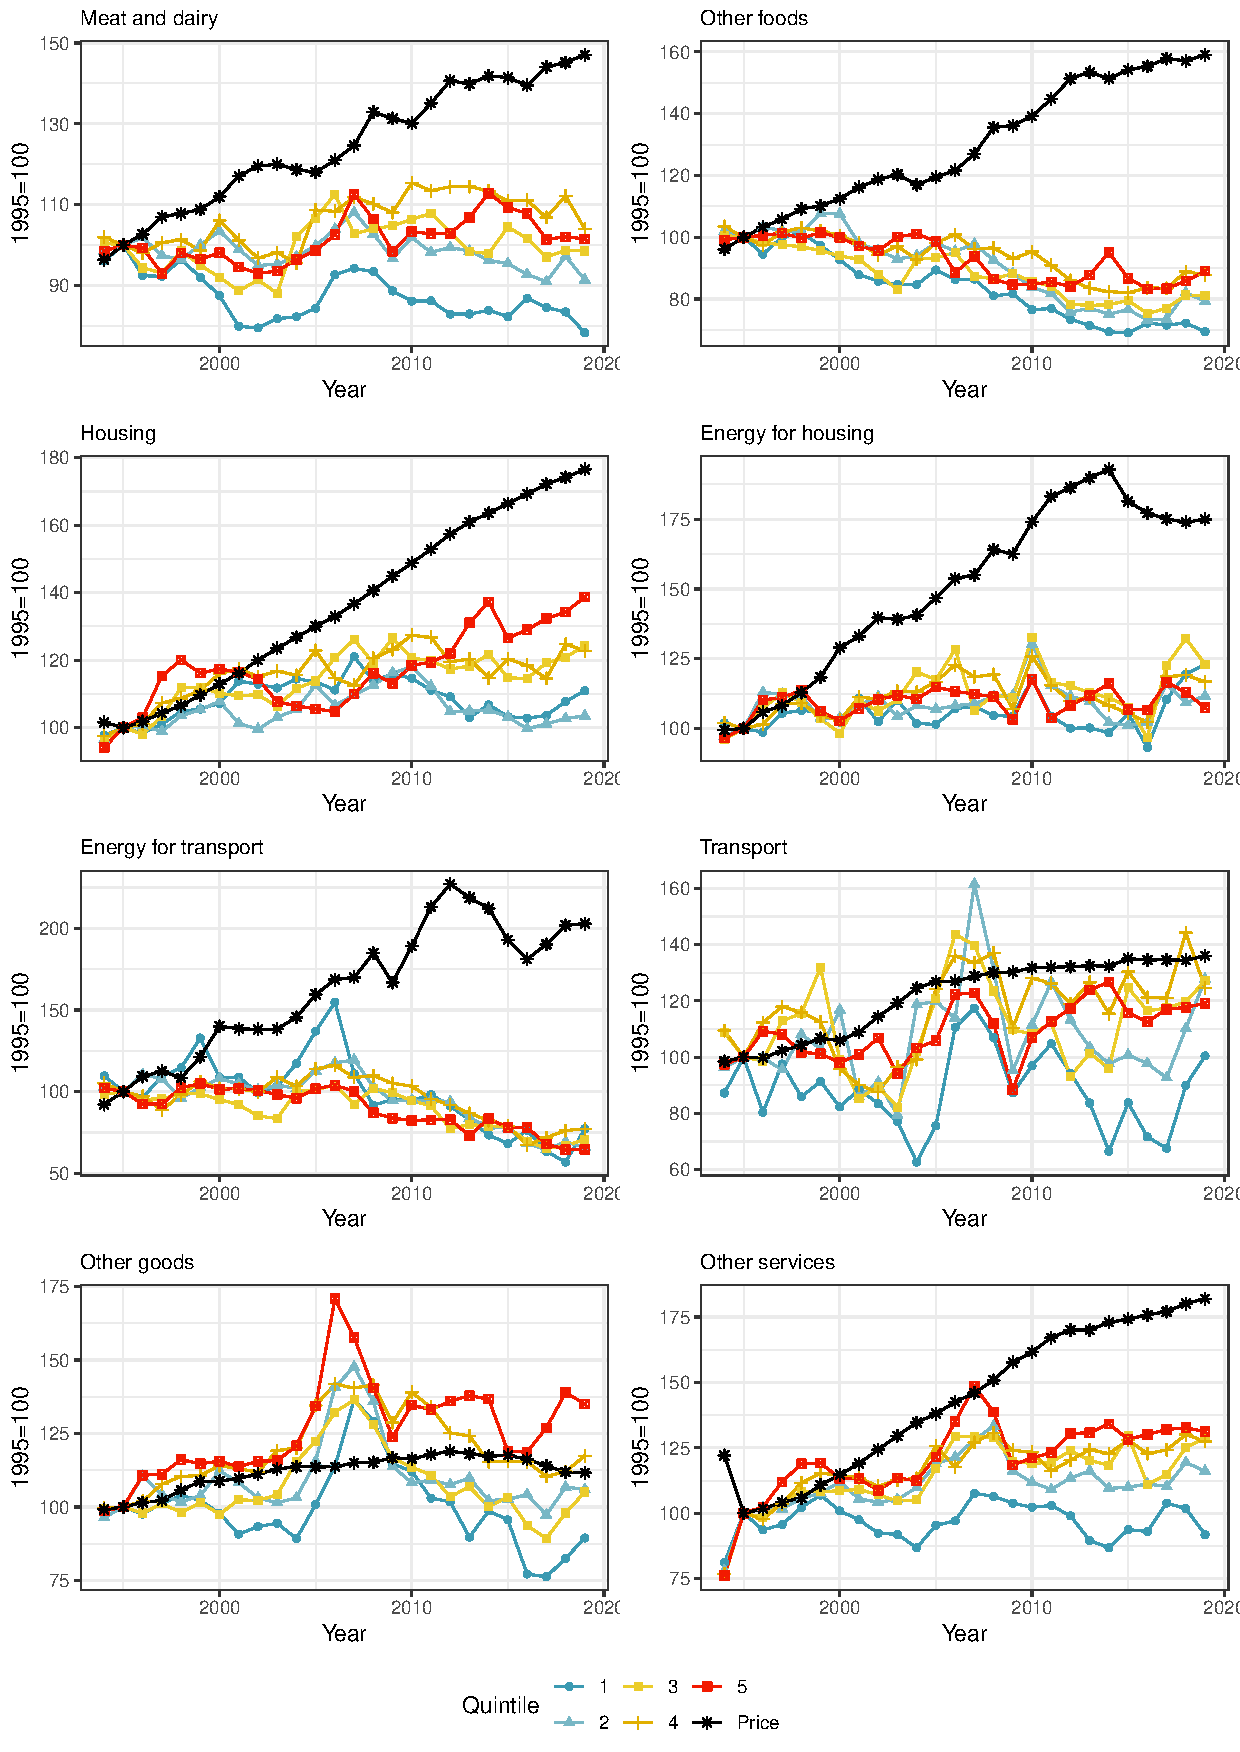
\includegraphics[width=.8\textwidth]{Figures/indexpricecons.pdf}
\captionsetup{singlelinecheck=off,size=scriptsize}
\setlength{\captionmargin}{10pt}
\caption*{
\textbf{Note:} Real consumption in 1995 prices}
\end{figure}

Except for the two energy goods, the price of housing has risen the most of the 8 consumption composites. Real consumption of housing has stayed approximately constant over the sample period for the two bottom quintiles, but has increased for the upper quintiles. However, the price index as well as real consumption of housing should be interpreted with caution, as it is calculated based on imputed rent. 

Energy for housing has risen sharply in price over the sample period, while real consumption has stayed approximately constant for all quintiles. This could reflect both that it is a necessity good or intra-category substitution towards cheaper energy forms. Towards the end of the period, there does seem to have been a price response, where real consumption increased as the price fell. Energy for transport has also increased significantly in price over the period, while real consumption has fallen. This could indicate both increased fuel efficiency in cars as well as a relatively price-elastic demand. 

The transport composite has seen a moderate price increase while real consumption has been volatile. In the period leading up to the financial crisis in 2008-2009, there was a sharp increase in real consumption for all goods, followed by a sharp decrease. Over the entire sample, consumption as increased mostly for the richer part of the population. For other goods, which almost hasn't increased in price during the period, real consumption has also been volatile, and increased sharply leading up to the financial crisis and falling sharply afterwards. Over the sample period, it increased mostly for the riches quintiles, while it fell for the poorest. This could be an indication that other goods could be a luxury good, as the rich has seen a relatively larger increase in total expenditure during the sample. For other services, the rich has also increased their real consumption relatively more than the poor. 




